\section{Comparing requests}\label{sec:requests}

The analysis that replaces both withdrawn rules compares what an observer of the
transcript actually receives: the requests, by content. This section defines
request signatures, resolves secret branches over the outcomes a secret can realise,
and proves noninterference, a leakage bound, results for coarser observers and a
completeness result.

\subsection{Request signatures and resolution}\label{sec:signatures}

\begin{definition}[Request signature]\label{def:signature}
The \emph{signature} of a region of a workflow is a list of nodes
\begin{align*}
\mathit{node} &::= \Call(m, \mathit{pieces}) \mid \Retry(n, \mathit{sig}) \mid
\Branch(g, \mathit{sig}, \mathit{sig}) \\
\mathit{piece} &::= \ptext(t) \mid \pvar(b) \mid \pres(p),
\end{align*}
where $m$ is a model identity, $\ptext(t)$ is static text as sent (template text and
literal arguments, with adjacent text merged), $\pvar(b)$ is a binding made outside
the region, identified by its declaration and with public content, and $\pres(p)$ is
the response of the call at position $p$ inside the region.
\end{definition}

A branch whose guard has public content contributes a $\Branch$ node with its
guard term. A branch whose guard reads secret content is \emph{resolved}. Because
only secrets and their endorsed copies carry secret content, and the \textsc{Call}
rule keeps both out of requests, every secret guard is a predicate of the secrets
alone. For a secret $s$ with declared bound $B$, the guards $\code{tokens}(s) \bowtie
k$ partition $[0, B]$ into intervals, and a boolean secret has two values. The
analysis evaluates each guard at every value that could change an outcome, collects
the outcome vectors that some value realises, and takes the product over
independent secrets. The resulting set $F$ is exactly the set of \emph{feasible}
outcome vectors. For $v \in F$, $\sigv{v}(c)$ is the signature of $c$ with every
secret guard resolved by $v$, that is, with the selected arm inlined, and
\[
k(c) = \bigl|\{\, \sigv{v}(c) : v \in F \,\}\bigr|
\]
is the number of distinct signatures. The implementation computes $k(c)$ up to the
normal forms of \cref{sec:coarser} for the observer the workflow declares.

\begin{figure}[t]
\centering
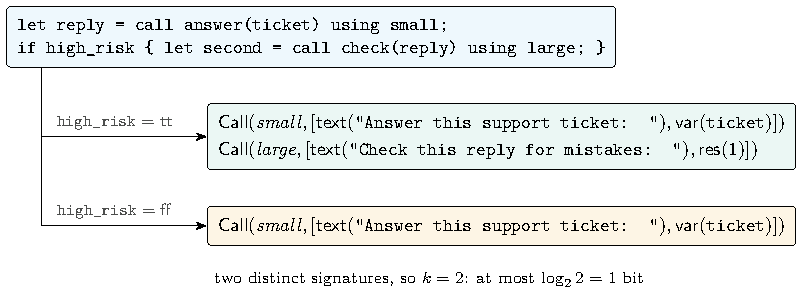
\includegraphics[width=\textwidth]{fig-resolution.pdf}
\caption{Resolution of the running example. The guard \code{high\_risk} reads secret
content, so the analysis inlines each arm the secret can select. The two resulting
signatures differ in their second call, so $k = 2$: the workflow is rejected with
\code{E236}, or accepted with a one-bit budget (\code{leaks 1}). The response of the first
call appears as $\pres(1)$, not as text, because its content is the same in both
executions whatever it is. (Diagram drawn in TikZ with the help of Claude, Anthropic.)}
\label{fig:resolution}
\end{figure}

\begin{example}\label{ex:triage-signature}
\Cref{fig:resolution} resolves \cref{fig:triage}. The first call contributes
\[
\Call(\mathit{small}, [\ptext(\code{"Answer this support ticket: "}), \pvar(\code{ticket})])
\]
to both resolutions. With $\code{high\_risk} = \mathsf{tt}$ the second call is inlined
with the piece $\pres(1)$ for \code{reply}; with $\mathsf{ff}$ nothing is. The two
signatures differ, so $k = 2$. The compiler's message in \cref{fig:triage} prints
exactly this difference.
\end{example}

\subsection{Noninterference}\label{sec:ni}

\begin{lemma}[Equal signatures, equal histories]\label{lem:equal}
Let $\sigv{v_1}(c_1) = \sigv{v_2}(c_2)$, where $v_i$ is the outcome vector of store
$\sigma_i$, and let $\sigma_1$ and $\sigma_2$ agree on every binding that occurs in a
$\pvar$ piece. Then for every tape and every common history, running $c_1$ from
$\sigma_1$ and $c_2$ from $\sigma_2$ under the global, model or request scheme extends
the history by the same events, and binds equal values at corresponding positions.
\end{lemma}

\begin{proof}[Proof sketch]
By induction on the signature. At a call, equal pieces denote equal text: $\ptext$
pieces directly, $\pvar$ pieces by hypothesis, and $\pres$ pieces by the induction
hypothesis. The same request therefore goes to the same model from the same
history, the scheme computes the same key, the tape supplies the same draw, and
$\Pi$ returns the same response. At a retry, equal bodies produce equal attempt
transcripts, and $V$ reads the same transcript and draw, so both executions stop
after the same attempt. A public branch reads equal values and takes the same arm.
A resolved branch inlines the arm that the store actually takes, since $v_i$ is
$\sigma_i$'s own outcome vector. The full proof is in \ref{app:proofs}.
\end{proof}

\begin{theorem}[Request-trace noninterference]\label{thm:ni}
If $k(c) = 1$, then $c$ is pointwise \code{trace}-noninterfering under the global,
model and request schemes, and hence $O$-noninterfering for every provider in
$\Prov$, every tokenizer, every envelope and every observer $O$ that is a function
of the history.
\end{theorem}

\begin{proof}
Take related stores $\sigma_1 \sim \sigma_2$ with outcome vectors $v_1, v_2$. Both
vectors are feasible, so $\sigv{v_1}(c) = \sigv{v_2}(c)$ when $k(c) = 1$. For the
whole workflow every $\pvar$ piece is a public input or a declassified value, on
which the stores agree. \Cref{lem:equal} with the empty history gives equal histories
on every tape, \cref{lem:coupling} turns this into equal distributions, and every
observer is a function of the history.
\end{proof}

No assumption about tokenizers is used. Equal histories contain equal request
texts, and any tokenizer bills equal texts equally; that is the practical
difference from comparing sizes, which is only as good as a tokenizer assumption
and, by \cref{thm:size-blind}, not even that good. In the terms of probabilistic
relational Hoare logic~\cite{barthe2009formal}, \cref{lem:equal} is a derivation
in which every provider call is related by the identity coupling on its draw. The
sampling rule that justifies such a step requires the two distributions to be equal
up to a bijection, and with the identity bijection they must be identical. Requests
with equal content satisfy this; requests with equal size do not, and read as such
a derivation the size rule applies the rule to two different distributions. More broadly, comparing two resolutions is a specialised form of
self-composition~\cite{Barthe2004SelfComposition,Terauchi2005Safety,Barthe2016ProductPrograms}
in which the product program never has to be built, because the signatures are
compared directly.

\subsection{Quantitative leakage}\label{sec:quantitative}

Rejecting every workflow with $k(c) > 1$ is too strict for workflows that must reveal
a little, such as a service tier that selects a larger model for paying
customers. A workflow may declare a budget \code{leaks} $b$, and it is accepted with
warning \code{W238} if $k(c) \leq 2^b$.

\begin{theorem}[Leakage bound]\label{thm:leakage}
For every provider in $\Prov$, every fresh keying scheme and every observer of the
history, together with the workflow's outputs and effects, the channel from the
secrets to the observer has min-capacity at most $\log_2 k(c)$. The bound holds for
any number of invocations with the same secrets and any public inputs, including
public inputs chosen adaptively from earlier observations.
\end{theorem}

\begin{proof}[Proof sketch]
Partition the secret assignments by the class of their signature; there are at
most $k(c)$ classes. By \cref{lem:equal}, two assignments in one class produce equal
histories on every tape and for every public input, since signatures are symbolic
in the public inputs. Outputs and effects are functions of public data and
responses, because the type system rejects any output or effect under a secret
program counter (\cref{fig:rules}). Each invocation's observation is therefore a
function of the class, the public inputs and the tape, and over adaptively chosen
invocations the whole observation sequence is a function of the class, the tapes
and the adversary's coins. The channel is a cascade whose first stage is a
deterministic map onto at most $k(c)$ classes. The min-entropy leakage of a cascade
is at most that of its first stage~\cite{espinoza2012min}, and for every prior the
min-entropy leakage of a channel with at most $k$ possible outputs is at most
$\log_2 k$~\cite[Theorem 1]{doychev2013cacheaudit}; see also~\cite{kopf2010vulnerability}.
\ref{app:proofs} gives the details.
\end{proof}

The argument follows Köpf and Basin's model of an adaptive attacker as a partition
of the secrets into classes the attacker cannot tell apart~\cite{kopf2007information},
with signature classes in place of observations. Counting observations would
be useless here, since the provider's noise gives every workflow with a call a vast
number of possible observations; that is why the interval bound of
\cref{sec:classical} is vacuous. The coupling removes the noise from the count.

\subsection{Coarser observers, and an unsound optimisation}\label{sec:coarser}

A bill does not record order, and a provider sees only its own requests. The
\emph{provider normal form} of a signature stably sorts, by provider, every maximal
run of calls none of which references another in the run, outside any retry body,
and rewrites $\pres$ references to follow the moved calls. The \emph{bill normal
form} sorts such runs by the full request.

\begin{theorem}[Coarser observers]\label{thm:observers}
If the provider (bill) normal forms of $\sigv{v}(c)$ agree for all feasible $v$, then
$c$ is pointwise \code{provider}- (\code{bill}-) noninterfering under the request
scheme, and hence \code{provider}- (\code{bill}-) noninterfering.
\end{theorem}

Under the request scheme a call's draw is keyed by its request and occurrence, not
by its position, so a stably sorted run sends the same multiset of requests and
each copy of a request receives the same response. Calls inside a retry body are
not reordered: the validator sees an attempt's transcript in order, and it may
depend on the order. An intermediate version of our analysis did reorder there. It
accepted a workflow for which, under the same seed, the runtime made one attempt
for one value of the secret and three for the other. The workflow is now a regression
test.

\subsection{Completeness relative to dead code}\label{sec:completeness}

\begin{theorem}[Relative completeness]\label{thm:completeness}
Suppose $\sigv{v_1}(c) \neq \sigv{v_2}(c)$ for feasible $v_1, v_2$, and every public
guard on the path to the first difference can go either way for some public inputs
and responses. Then some provider in $\Prov$ distinguishes the two secrets. For
$k(c)$ classes, some provider and prior attain the bound of \cref{thm:leakage}.
\end{theorem}

\begin{proof}[Proof sketch]
Choose public inputs that are distinct fresh strings, and a provider whose responses
are fresh strings encoding the request and the draw, with a validator that always
fails. Rendering signatures to histories is then injective, and the histories agree
up to the first difference by \cref{lem:equal}.
\end{proof}

A rejection is therefore justified, except when the difference sits under a public
guard that can never go the relevant way. One consequence concerns two different
public variables of equal declared length. A size-based rule accepts a branch that
sends one in each arm; the content rule rejects it, and \cref{thm:completeness} says
the rejection is required, because the variables can hold different text and some
provider answers them differently.
